    
    \clearpage
    \begin{table}[H]
    \centering
		\begin{tabular}{|x{\textwidth}|}
			\hline 
            \MakeUppercase{\csuniversidad} \\
            \\
            \begin{minipage}{.3\textwidth}
				
\includegraphics[width=\textwidth]{../imgs/cs2}
	        \end{minipage} \\
        	\\
            \textbf{\MakeUppercase{\csepcc}} \\
            \MakeUppercase{\csfacultad} \\
            \MakeUppercase{\csdepartamento} \\
			\hline 
		\end{tabular}
	\end{table}


    %\begin{figure}				
	%			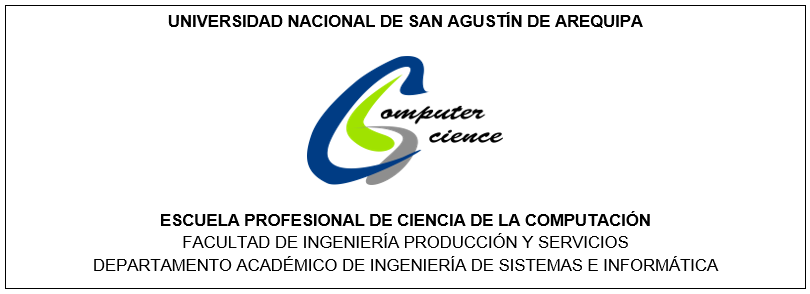
\includegraphics[width=\textwidth]{../imgs/cs}
	%\end{figure}
    \centering
    \textbf{INFORME DE RESULTADOS}    
        
    \begin{table}[H]
    \centering
		\begin{tabular}{|p{4cm}|p{2cm}|}
			\hline 
			\textbf{Nota máxima} & 18   \\
			\hline 
            \textbf{Nota mínima} & 2   \\
			\hline
			\textbf{Nota promedio} &  13   \\
			\hline 
		\end{tabular}
	\end{table}	
      
    \begin{flushleft}
    En la Figura \ref{fig:hist_EP1}, detallamos el histograma de frecuencias de las
    notas por grupo y en la Figura \ref{fig:hist_all_EP1}, mostramos el consolidado. 
    \end{flushleft}

    \begin{figure}[H]	
    \centering 		
				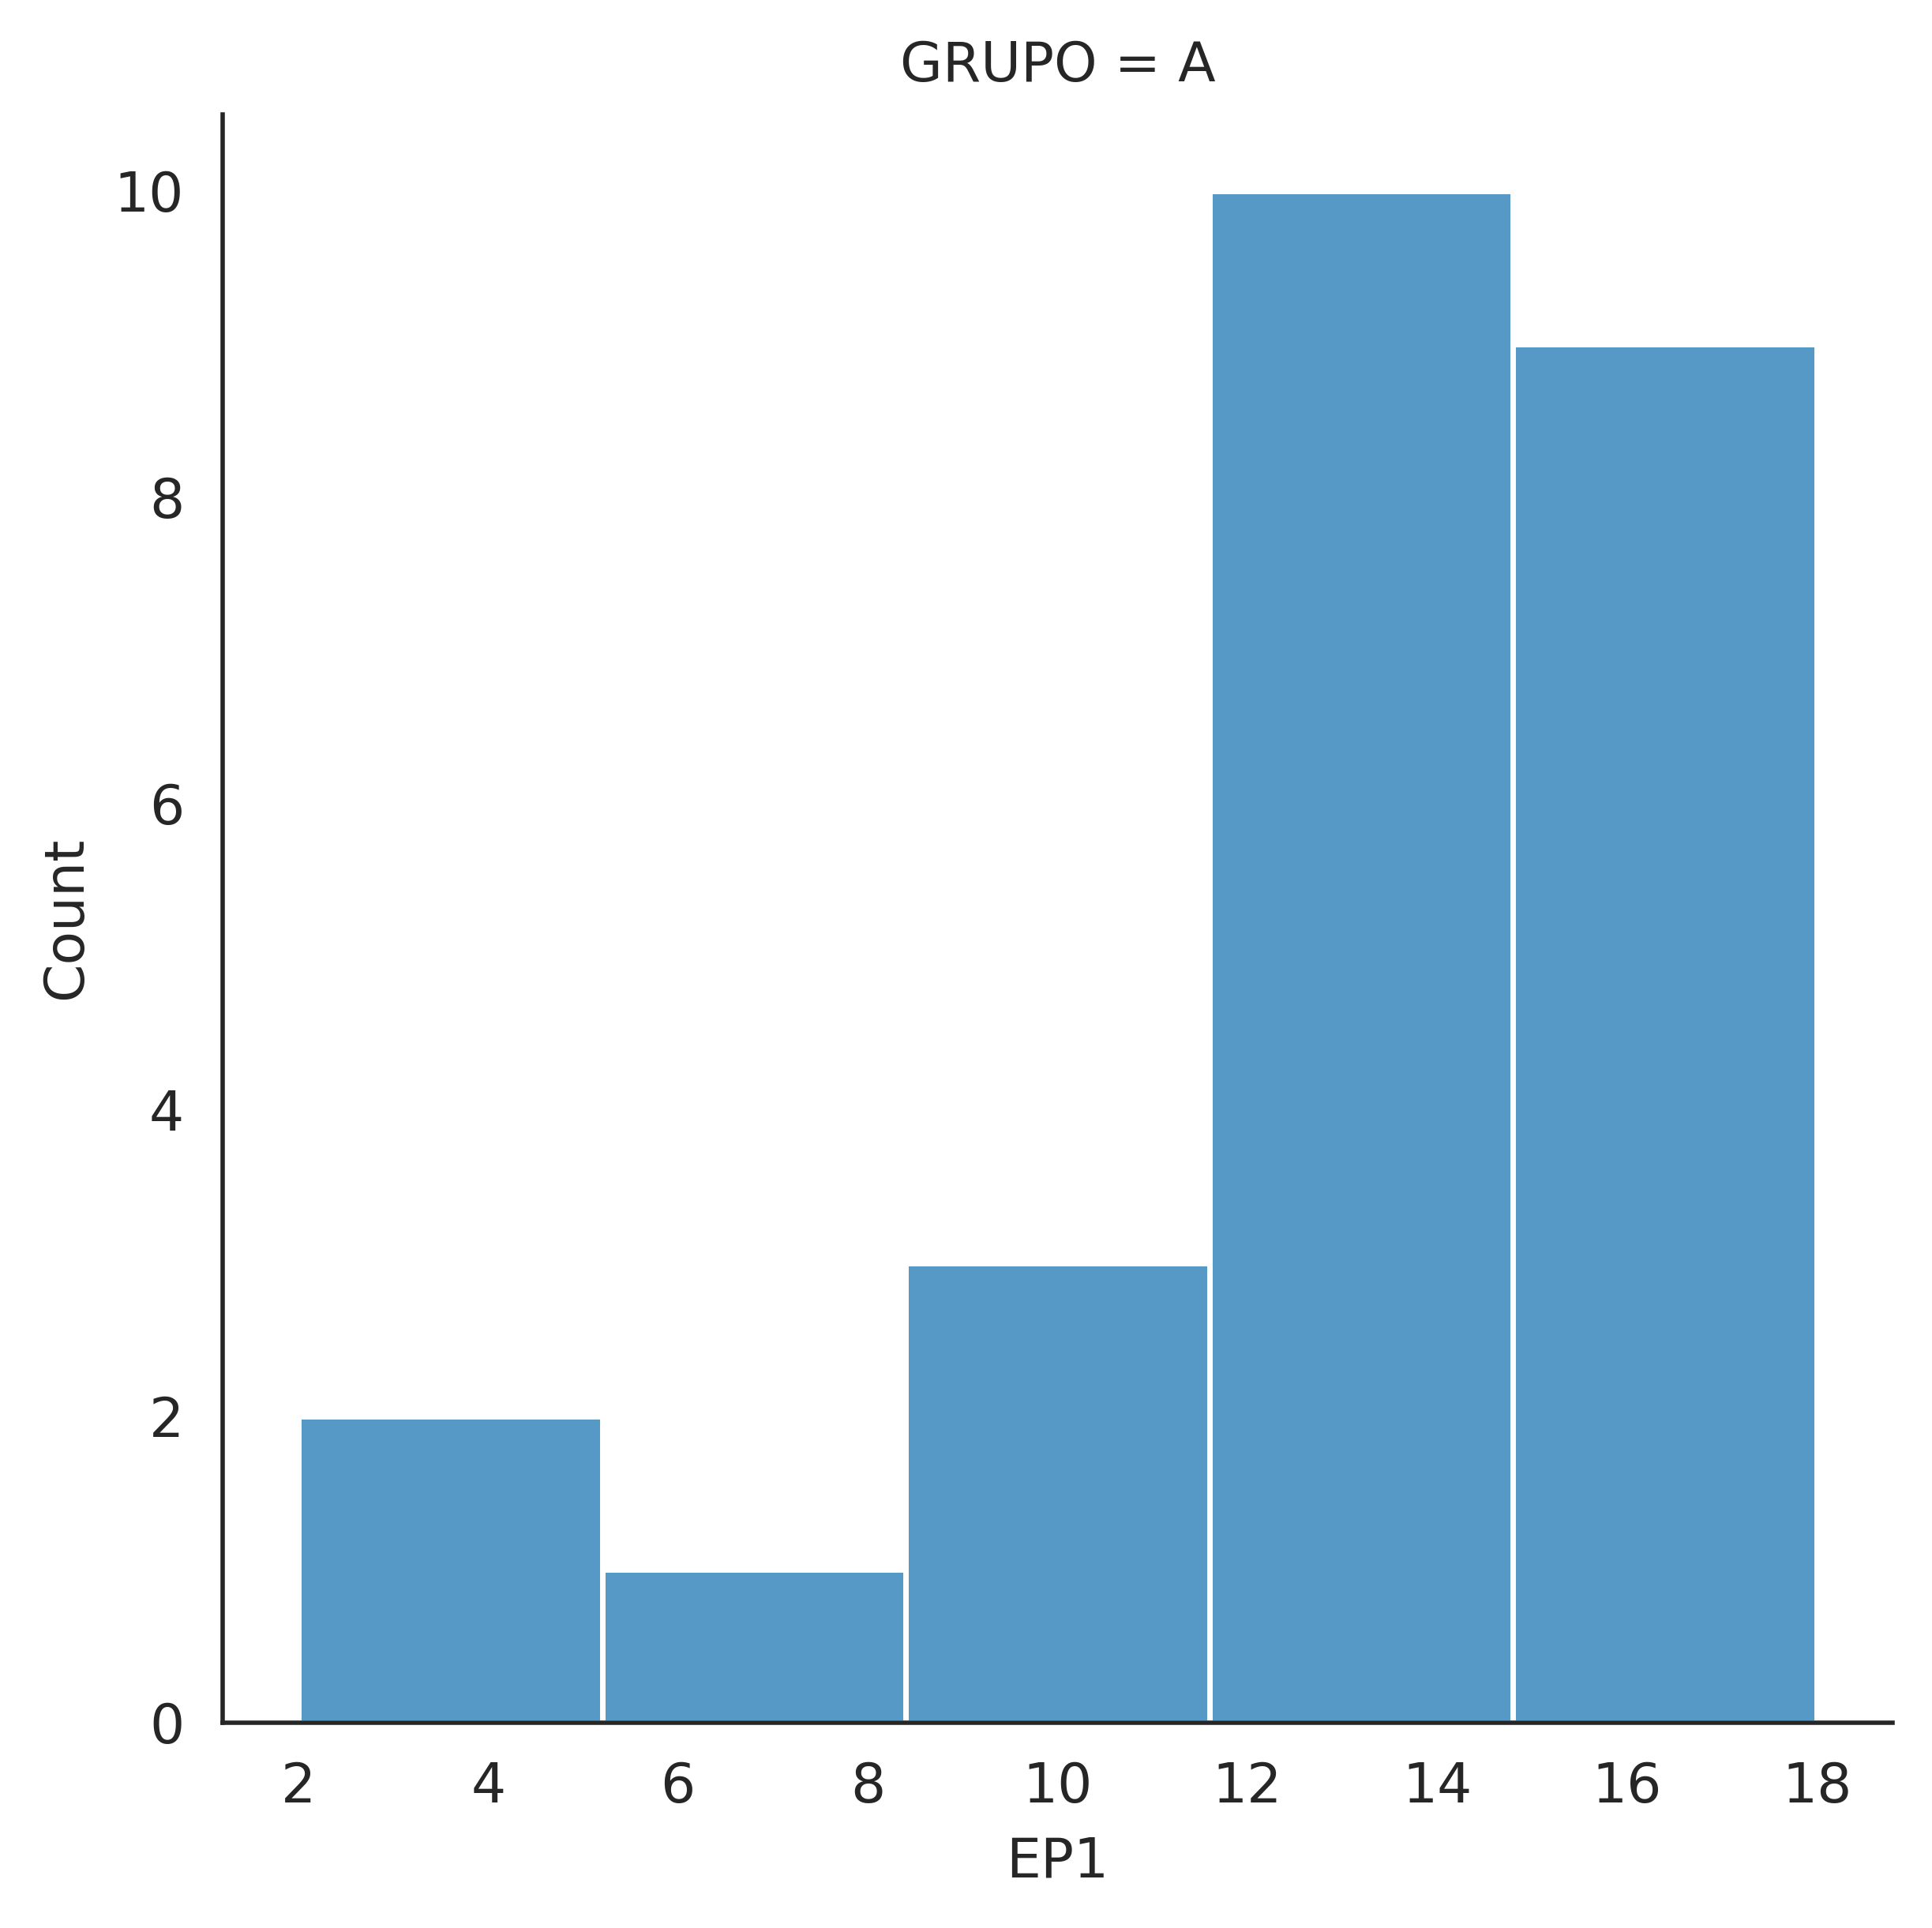
\includegraphics[width=0.6\textwidth]{../imgs/hist_EP1.png}
                \caption{Histograma de notas.}
                \label{fig:hist_EP1}
	\end{figure}

    \begin{figure}[H]	
    \centering 		
				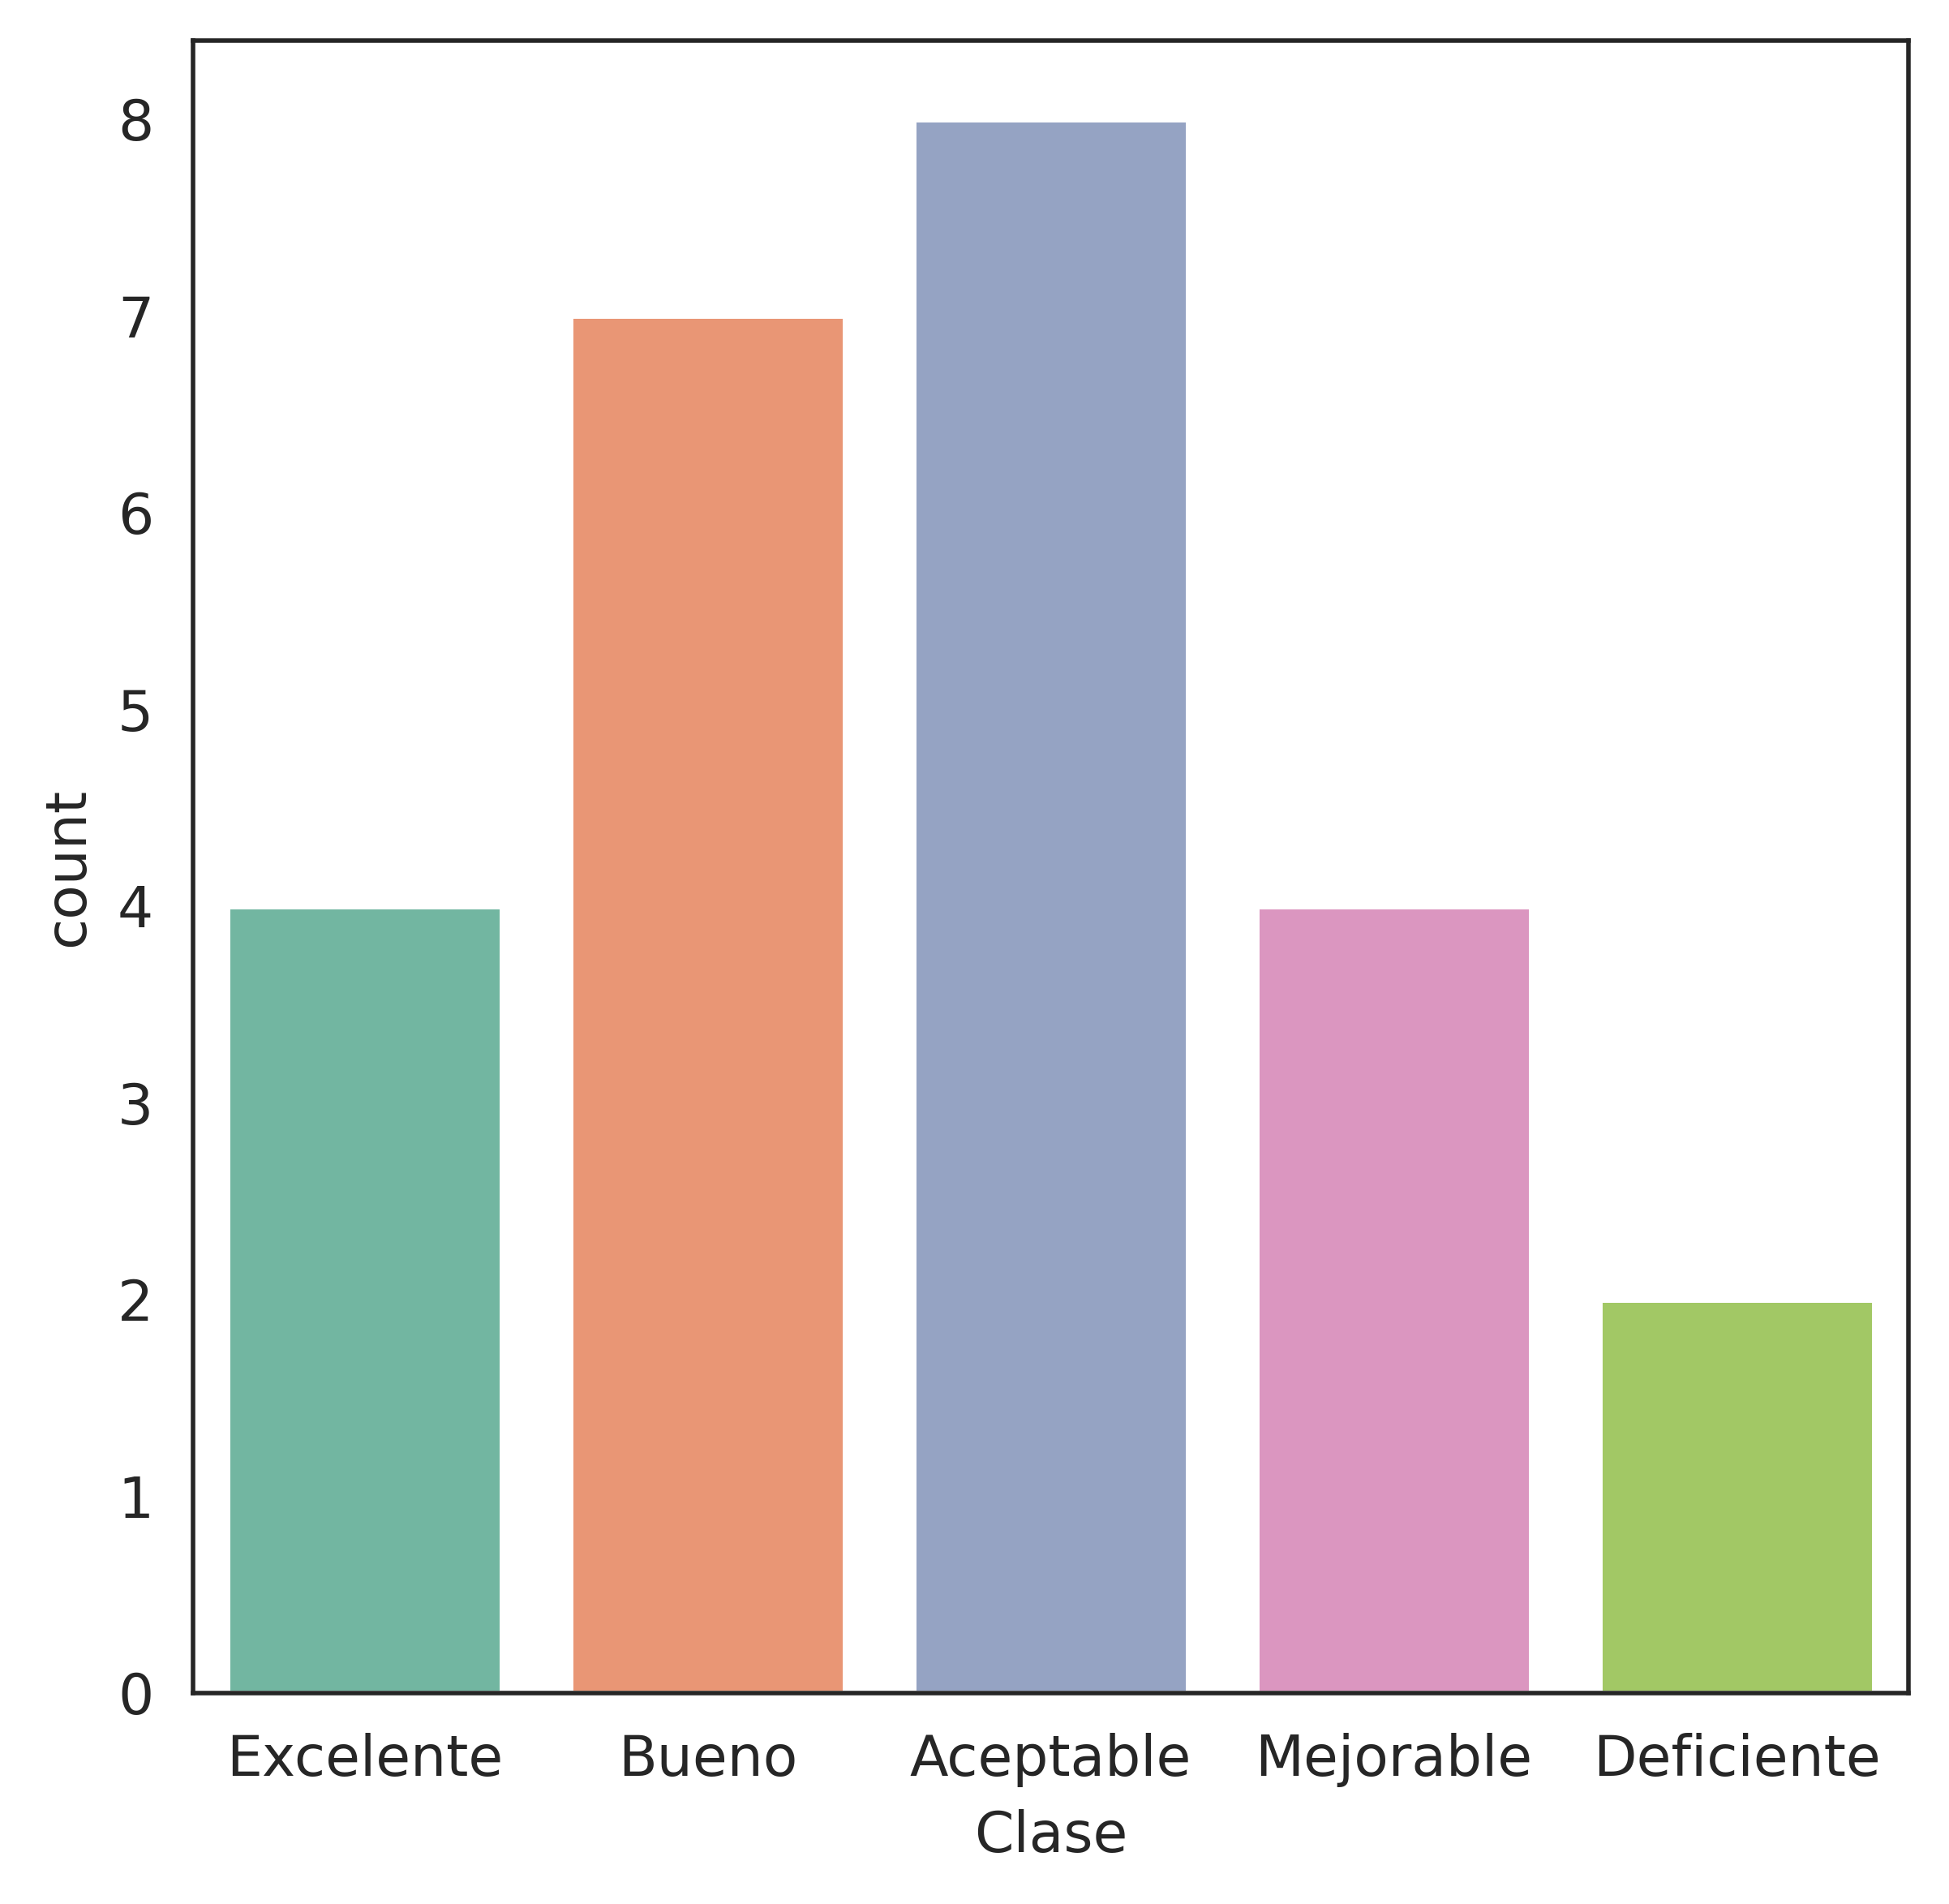
\includegraphics[width=0.6\textwidth]{../imgs/hist_all_EP1.png}
                \caption{Histograma de notas (consolidado). Excelente (nota $\geq$ 17), Bueno (14 $\leq$ nota $\leq$ 16), Aceptable (11 $\leq$ nota $\leq$ 13), Mejorable (07 $\leq$ nota $\leq$ 10), Deficiente ( nota $\leq$ 06)}
                \label{fig:hist_all_EP1}
	\end{figure}
      

        \begin{table}[H]
        \centering
            \caption{Notas del grupo A.}
            \begin{tabular}{|c|p{10cm}|c|}
                \hline 
                \textbf{CUI} & \textbf{ALUMNO} & \textbf{NOTA}  \\ \hline
        20153695 & APAZA CHAVEZ MARIA LOURDES & 15 \\ \hline 
            20143484 & AZA/MAMANI NICOLL DEL ROSARIO & 4 \\ \hline 
            20123493 & BARRIOS/CORNEJO SELENE & 14 \\ \hline 
            20123377 & BUSTINZA/CORNEJO ALEJANDRA PAMELA & 12 \\ \hline 
            20160748 & CESPEDES/FUENTES RENATO GONZALO & 18 \\ \hline 
            20143490 & CHUCTAYA/ELME MILAGROS & 9 \\ \hline 
            20132402 & CRUZ/MAMANI MILAGROS CELIA & 10 \\ \hline 
            20163436 & CUEVA/FLORES JONATHAN BRANDON & 12 \\ \hline 
            20052826 & ESPINEL QUISPE INGRID SALLY & 12 \\ \hline 
            20170734 & FERNANDEZ/MAMANI BRAYAN GINO & 14 \\ \hline 
            20173462 & GARCIA/DIAZ GERMAN FLAVIO & 16 \\ \hline 
            20163427 & GOMEZ/CONTRERAS JUNIOR VALENTIN & 8 \\ \hline 
            20143482 & GUTIERREZ/GUTIERREZ DIEGO ANTONY & 12 \\ \hline 
            20170732 & HERMOZA/LOAYZA MIGUEL ANGEL & 18 \\ \hline 
            20170735 & HERRERA/COOPER MIGUEL ALEXANDER & 13 \\ \hline 
            20160746 & INCA/CHIPANA GUSTAVO HERNAN & 10 \\ \hline 
            20151124 & NIFLA/CATASI WILLIAMS FIDEL & 13 \\ \hline 
            20160759 & OXA/CACYA SHIRLEY MICHELLE & 17 \\ \hline 
            20160750 & PANIBRA/MAMANI THALES GONZALO & 12 \\ \hline 
            20041749 & PILCO/PANCCA LUZ MARINA & 17 \\ \hline 
            20173453 & QUISPE/MENOR HERMOGENES & 16 \\ \hline 
            20153709 & QUISPE/QUISPE YARA JEANETTE & 12 \\ \hline 
            20110202 & TACORA/CRUZ RICHARD JAVIER & 2 \\ \hline 
            20173449 & TORRES/RODRIGUEZ JAIME FRANCISCO & 16 \\ \hline 
            20170737 & VICENTE/CASTRO RENZO OMAR & 16 \\ \hline 
            		
            \end{tabular}
        \end{table}	
        